\subsection{premi/client/fallback}
\begin{figure}[H]
\begin{center}
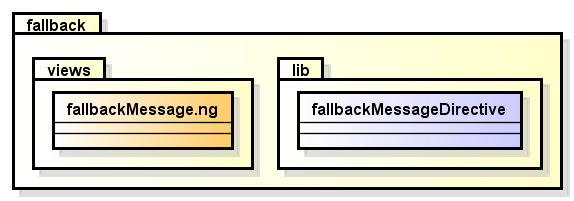
\includegraphics[scale=0.70]{img/diapkg/fallback.png}
\caption{Diagramma della classe premi/client/fallback}
\end{center}
\end{figure}

%-------  diagramma di un template %
\subsubsection{premi/client/fallback/views/fallbackMessage.ng}

\begin{description}
%-------  descrizione del template%
\item[Descrizione] \hfill
	template della vista associato alla direttiva \textit{fallbackMessageDirective} che permette di visualizzare il logo e di personalizzare il messaggio che deve essere visualizzato nella navbar.
\end{description}

%-------  diagramma di un template %
\subsubsection{premi/client/fallback/lib/fallbackMessageDirective}

\begin{description}
%-------  descrizione del template%
\item[Descrizione] \hfill
	direttiva che include la vista \textit{fallbackMessage.ng} e permette con il tag html$_G$ \textit{fallback-message} di mostrare un messaggio nella navbar all'utente.
\end{description}

